\section{Conformal Symmetry in Field Theories}

At a critical point, the correlation length diverges:
\[
    \xi\rightarrow\infty.
\]
In the language of Quantum Field Theory (QFT), \uline{the inverse of the correlation length corresponds to the mass of the lightest excitation in the spectrum} (\(m \sim \xi^{-1}\)), which defines the \textbf{energy gap} above the vacuum. When \(\xi \rightarrow \infty\), this mass gap vanishes, resulting in a \textit{gapless} or \textit{massless} theory (analogous to Quantum Electrodynamics, where the fundamental photon is massless). Since a non-zero mass introduces a fundamental length or energy scale, a massless theory cannot distinguish between different observation scales. Therefore, \uline{a diverging correlation length inherently implies that the theory is \textit{scale invariant}}.

As a consequence, the system becomes invariant under global scale transformations of the spacetime coordinates (including time):
\[
    x^{\mu}\rightarrow\lambda x^{\mu}.
\]
Under this rescaling, the fundamental objects of the theory (the local fields, regardless of their scalar, vector, or tensor nature) transform according to their \textbf{scaling dimension} \(\Delta\):
\[
    \phi(x)\rightarrow\lambda^{-\Delta}\phi(\lambda x).
\]
In general, the space of all possible fields can be thought of as a vector space. It is always possible to select a preferred basis of fields such that every element has a definite scaling dimension. Any arbitrary field can then be expressed as a linear combination of these basis fields, a procedure conceptually identical to finding the eigenoperators of the Renormalization Group (RG) flow.

Away from criticality, correlation functions typically exhibit an exponential decay governed by the correlation length, \(\sim e^{-|x|/\xi}\). However, at a critical point (\(\xi \rightarrow \infty\)), this exponential suppression factor evaluates to \(1\). Consequently, the scale invariance rigidly dictates that correlation functions must exhibit a pure power-law behavior:
\[
    \langle\phi(x)\phi(0)\rangle\sim\frac{1}{|x|^{2\Delta}}.
\]

It is therefore very important to deepen our knowledge of scale transformations. As we shall see, a crucial result (the classical Polyakov theorem, a powerful extension of Noether's theorem) states that, under quite general assumptions, scale invariance in field theory is almost always enhanced to a much larger symmetry: \textit{conformal invariance}. Thus, the first necessary step is to formally understand what conformal invariance is and how it governs the theory.

\subsection{Conformal Transformations}
General coordinate transformations \(x\rightarrow x^{\prime}\) change the metric tensor as
\[
    g_{\mu\nu}^{\prime}(x^{\prime})=\frac{\partial x^{\prime\lambda}}{\partial x^{\mu}}\frac{\partial x^{\prime\sigma}}{\partial x^{\nu}}g_{\lambda\sigma}(x).
\]
Conformal transformations are coordinate transformations of type
\[
    \frac{\partial x^{\prime\lambda}}{\partial x^{\mu}}=\Omega(x)g^{\lambda}_\mu,
\]
preserving the metric up to a local rescaling \(\mathrm{d}s^{\prime 2} = \Omega^{2}(x)\mathrm{d}s^2 \):
\[
    g_{\mu\nu}^{\prime}(x^{\prime})=\Omega^{2}(x)g_{\mu\nu}(x), \quad \Omega^{2}(x)=e^{f(x)}>0.
\]

Physically, this represents a strictly \textit{local} rescaling of the coordinates. Unlike a global scale transformation that stretches the entire space uniformly, a conformal transformation allows the scale factor \(\Omega(x)\) to vary from point to point. Geometrically, if one imagines a coordinate grid, this operation allows you to fix a point and locally ``inflate'' or ``deflate'' the grid around it. The coordinates change scale in different ways at different positions in space, but without arbitrarily mixing the coordinate axes in a way that would alter the angles between intersecting lines.

\begin{figure}[H]
    \centering

    % --- MINIPAGE 1: Global Conformal Transformation ---
    \begin{minipage}{0.48\textwidth}
        \centering
        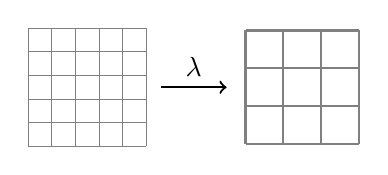
\begin{tikzpicture}[scale=1.2]
            % Original grid (dense)
            \draw[step=0.25, gray, thin] (0,0) grid (1.25,1.25);

            % Global transformation arrow
            \draw[->, thick] (1.4, 0.625) -- (2.1, 0.625) node[midway, above] {$\lambda$};

            % Rescaled grid (zoomed, perfectly centered and bounded)
            \begin{scope}[shift={(2.3, 0.025)}]
                \draw[step=0.4, gray, thick] (0,0) grid (1.201, 1.201);
            \end{scope}
        \end{tikzpicture}
        \caption{Global scale transformation: the grid is scaled uniformly at every point by a constant factor $\lambda$.}
        \label{fig:global_scale}
    \end{minipage}\hfill
    % --- MINIPAGE 2: Local Conformal Transformation ---
    \begin{minipage}{0.48\textwidth}
        \centering
        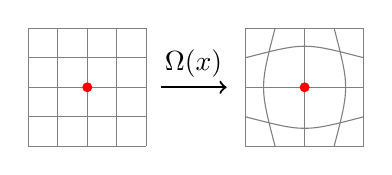
\begin{tikzpicture}[scale=1.2]
            % Original grid
            \draw[step=0.3125, gray, thin] (0,0) grid (1.25,1.25);
            % Central point
            \fill[red] (0.625, 0.625) circle (1.5pt);

            % Local transformation arrow
            \draw[->, thick] (1.4, 0.625) -- (2.1, 0.625) node[midway, above] {$\Omega(x)$};

            % Locally "inflated" grid (Simulated barrel distortion)
            % Outer border
            \draw[gray, thin] (2.3,0) rectangle (3.55,1.25);

            % Deformed horizontal lines
            \draw[gray, thin] (2.3, 0.3125) .. controls (2.925, 0.15) .. (3.55, 0.3125);
            \draw[gray, thin] (2.3, 0.625) -- (3.55, 0.625); % Invariant central line
            \draw[gray, thin] (2.3, 0.9375) .. controls (2.925, 1.1) .. (3.55, 0.9375);

            % Deformed vertical lines
            \draw[gray, thin] (2.6125, 0) .. controls (2.45, 0.625) .. (2.6125, 1.25);
            \draw[gray, thin] (2.925, 0) -- (2.925, 1.25); % Invariant central line
            \draw[gray, thin] (3.2375, 0) .. controls (3.4, 0.625) .. (3.2375, 1.25);

            % Central point after transformation
            \fill[red] (2.925, 0.625) circle (1.5pt);
        \end{tikzpicture}
        \caption{Local conformal transformation: the grid undergoes a local ``inflation'' determined by the position-dependent factor $\Omega(x)$.}
        \label{fig:local_scale}
    \end{minipage}

\end{figure}

This mechanism becomes particularly interesting when applied to a spacetime characterized by a \textbf{flat metric}, where the original \(g_{\mu\nu}\) is a constant matrix independent of the position \(x\). In a \(D\)-dimensional flat spacetime with metric
\[
    g_{\mu\nu} = \begin{dcases}
        \delta_{\mu\nu} = \text{ diag}(1,1,\dots,1) \text{ if Euclidean,} \\
        \eta_{\mu\nu} = \text{ diag}(-1,1,\dots,1) \text{ if Minkowskian,}
    \end{dcases}
\]
the \textbf{conformal condition} can be explicitly written as:
\begin{equation}
    \partial_{\mu}x^{\prime\rho}\partial_{\nu}x^{\prime\sigma}g_{\rho\sigma}=\Omega^{2}(x)g_{\mu\nu}.
    \label{eq:conformal_condition}
\end{equation}
Thus if we have already Wick rotated to Euclidean signature, we will be working with the Euclidean metric \(\delta_{\mu\nu}\), if not, we will be working with the Minkowski metric \(\eta_{\mu\nu}\). In any case, the conformal condition can be expressed as shown above, where \(g_{\mu\nu}\) is the appropriate metric for the signature we are working with.

\subsection{Conformal Killing Equation}

Since we are interested in finding the Lie algebra of this transformations group, thus it is convenient to consider infinitesimal transformations. For an infinitesimal transformation we can write
\[
    x^{\prime\mu}=x^{\mu}+\epsilon^{\mu}(x),
\]
and, since \(\Omega^{2}(x)\) is a positive function, we choose to write it as the exponential of another function \(f(x)\) (this is just a convenient parametrization, not a restriction):
\[
    \Omega^{2}(x)=e^{f(x)}\simeq 1+f(x)+\dots
\]
Taking the conformal condition \eqref{eq:conformal_condition} and inserting the infinitesimal transformation (recognizing that the l.h.s. is the metric in the new coordinates, i.e. \(g_{\mu\nu}^{\prime}\)), we get
\[
    g_{\mu\nu}^{\prime}=g_{\mu\nu}+(\partial_{\mu}\epsilon_{\nu}+\partial_{\nu}\epsilon_{\mu}),
\]
and now expanding \(g_{\mu\nu}^{\prime} = e^{f(x)}g_{\mu\nu}\) to first order in \(\epsilon\), we get
\[
    \partial_{\mu}\epsilon_{\nu}+\partial_{\nu}\epsilon_{\mu}=f(x)g_{\mu\nu}.
\]
We now take the trace of both members, multiplying by \(g^{\mu\nu}\) (saturting the indices), getting to
\[
    f(x)=\frac{2}{D}\partial_{\sigma}\epsilon^{\sigma}(x),
\]
which implies that the function \(f(x)\) is determined by the divergence of \(\epsilon^{\mu}(x)\). Inserting this back into the previous equation we get
\begin{equation}
    \partial_{\mu}\epsilon_{\nu}+\partial_{\nu}\epsilon_{\mu}=\frac{2}{D}(\partial \cdot \epsilon)g_{\mu\nu}.
    \label{eq:conformal_killing_equation}
\end{equation}
This is the conformal Killing equation, which is the fundamental equation defining the conformal Killing vectors \(\epsilon^{\mu}(x)\) that generate the conformal transformations. The solutions to this equation will give us the explicit form of the infinitesimal conformal transformations in flat spacetime.

\subsubsection{Solution of Conformal Killing Equation}
To explicitly solve the conformal Killing equation, one can apply a standard tensorial manipulation. By taking a further derivative of both sides, one obtains an equation with three spacetime indices. By cyclically permuting these indices to generate three distinct equations (adding the first two and subtracting the third) one can isolate the second derivatives of the displacement vector \(\epsilon(x)\).

After performing these algebraic steps, one finds that for spacetime dimensions \(D > 2\), the second derivatives of the scalar function \(f(x)\) must strictly vanish (\(\partial_\mu \partial_\nu f = 0\)). This implies that \(f(x)\) can be at most a linear function of the coordinates. Since \(f(x)\) is defined through the first derivative of \(\epsilon(x)\), it naturally follows that the third derivatives of \(\epsilon(x)\) must also vanish. Consequently, the components of \(\epsilon^\mu(x)\) are restricted to be at most \textit{quadratic} polynomials in the coordinates.

Indeed, for \(D>2\) the general solution for \(\epsilon(x)\) is precisely quadratic in \(x^{\mu}\), and it takes the exact form:
\[
    \epsilon^{\mu}(x)=a^{\mu}+{\omega^{\mu}}_{\nu}x^{\nu}+\lambda x^{\mu}+(b\cdot x)x^{\mu}-\frac{1}{2}x^{2}b^{\mu}.
\]
If we now restrict the form of the solution, we can get some informations about the structure of the conformal group. In particular, we can identify four different types of transformations, based on the parameters appearing in the solution:
\begin{itemize}
    \item \textbf{Translations} \(x^{\prime\mu}=x^{\mu}+a^{\mu}\): these are the simplest transformations, corresponding to a uniform shift of the coordinates by a constant vector \(a^{\mu}\).
    \item \textbf{Rotations} \(x^{\prime\mu}=x^{\mu}+{\omega^{\mu}}_{\nu}x^{\nu}\): this comes from the fact that we can always decompose the transformationmatrix into a symmetric and an antisymmetric part, and the latter corresponds to rotations.
    \item \textbf{Dilatations} \(x^{\prime\mu}=(1+\lambda)x^{\mu}\): this corresponds to an infinitesimal scaling of the coordinates (inflation or deflation), and it is indeed proportional to the coordinates themselves. This is the symmetric part we cited before, which is not a rotation but a scaling. It is an important transformation, since it is related to the scale invariance of the theory, and it is peculiar among the conformal transformations.
    \item \textbf{Special conformal transformations} \(x^{\prime\mu}=x^{\mu}+2(b\cdot x)x^{\mu}-b^{\mu}x^{2}\): these are the most non-trivial transformations, featuring a quadratic dependence on the coordinates. It is a \(D\)-parameter family of transformations (which reduces to 4 parameters in \(D=4\) dimensions), parameterized by the constant vector \(b^{\mu}\). Geometrically, this complex non-linear transformation can always be gracefully decomposed into a sequence of three fundamental operations: an inversion (\(x^{\mu} \rightarrow x^{\mu}/x^{2}\)), followed by a constant translation by the vector \(b^{\mu}\), and finally a second inversion.
\end{itemize}
The first two types of transformations (translations and rotations) are the usual Poincar\'e transformations, which are symmetries of any relativistic field theory. The last two types (dilatations and special conformal transformations) are additional symmetries that arise in scale-invariant theories, and they are responsible for the enhancement from scale invariance to full conformal invariance.

We already know the form of the generators of translations and rotations, since they are the usual ones, and they give us meaningful information about the structure of the theory of a Poincar\'e invariant QFT. We are here considering systems at criticality, which are scale invariant, thus it seems natural to expect that the generators of dilatations will also give us important information about the structure of the theory at criticality. Finally, the generators of special conformal transformations are the most non-trivial ones, and they are responsible for the full conformal symmetry of the theory, even if now we do not have a clear physical intuition about their meaning, but they are crucial for the structure of the conformal group and for the constraints that conformal invariance imposes on the theory.

Considering the application of these transformation on generic functions of the coordinates, we can obtain the form of the \textbf{generators}
\begin{itemize}
    \item \textbf{Translations}: \(P_{\mu}=-i\partial_{\mu}\), which is the usual generator of translations in field theory, corresponding to the momentum operator.
    \item \textbf{Rotations}: \(L_{\mu\nu}=i\epsilon_{\mu\nu\rho\sigma}x^{\rho}\partial^{\sigma}\), which is the usual generator of rotations (angular momentum) in field theory, corresponding to the angular momentum operator.
    \item \textbf{Dilatations}: \(D=-ix_{\mu}\partial^{\mu}\), which is the generator of dilatations (scale transformations) in field theory, and it is related to the scaling dimension of fields and operators in the theory.
    \item \textbf{Special conformal transformations}: \(K_{\mu}=-i(2x_{\mu}x^{\nu}\partial_{\nu}-x^{2}\partial_{\mu})\), which is the generator of special conformal transformations in field theory; we do not have a simple physical interpretation for this generator, but its importance will become clear when we discuss the structure of the conformal group.
\end{itemize}

\subsection{Conformal Algebra}

The generators of the first two types satisfy the usual roto-translation (Poincar\'e) algebra:
\begin{equation}
    \begin{dcases}
        [P_{\mu},P_{\nu}]            =0,                                               \\
        [P_{\rho},L_{\mu\nu}]        =\delta_{\rho\mu}P_{\nu}-\delta_{\rho\nu}P_{\mu}, \\
        [L_{\mu\nu},L_{\rho\sigma}]  =\delta_{\nu\rho}L_{\mu\sigma}+\delta_{\mu\sigma}L_{\nu\rho}-\delta_{\mu\rho}L_{\nu\sigma}-\delta_{\nu\sigma}L_{\mu\rho},
    \end{dcases}
    \label{eq:conformal_algbra_poincare}
\end{equation}
but now also the commutations with the dilatation operator \(D\) have to be added:
\begin{equation}
    \begin{dcases}
        [D,P_{\mu}]     =P_{\mu}, \\
        [D,L_{\mu\nu}]  =0,
    \end{dcases}
    \label{eq:conformal_algbra_dilatation}
\end{equation}
and finally those involving the special conformal transformations \(K_{\mu}\):
\begin{equation}
    \begin{dcases}
        [K_{\mu},K_{\nu}]=0,                                                   \\
        [K_{\rho},L_{\mu\nu}]=\delta_{\rho\mu}K_{\nu}-\delta_{\rho\nu}K_{\mu}, \\
        [K_{\mu},P_{\nu}]=2(\delta_{\mu\nu}D-L_{\mu\nu}),                      \\
        [D,K_{\mu}]=-K_{\mu}.
    \end{dcases}
    \label{eq:conformal_algbra_special_conformal}
\end{equation}
Note, in particular, that the rotation (spin) operator and the dilatation one commute, which means that we can find a basis of local fields that diagonalizes both operators simultaneously (this should not come as a surprise, since this two transformations are built from the symmetryc and antisymmetric parts of the general infinitesimal transformations).

This algebra is isomorphic to \(\mathfrak{so}(D+1,1)\) and the corresponding conformal group is \(SO(D+1,1)\) in euclidean spacetime (it would become \(SO(D,2)\) if a Minkowski metric is adopted instead). In any case, it is a group with \((D+1)(D+2)/2\) parameters.
Physically, every parameter of the symmetry group translates into a mathematical constraint that the Lagrangian (or the correlation functions) of the theory must satisfy. As a general rule, the larger the symmetry group, the tighter the constraints imposed on the theory.

For example, in \(D=4\) dimensions, requiring standard Poincar\'e invariance imposes 10 constraints on the theory (corresponding to the 10 generators of spacetime translations and Lorentz rotations). However, if we upgrade our requirement to full conformal invariance, the parameters of the conformal group become 15. Therefore, the Lagrangian is subjected to 15 strict constraints: the original 10 from the Poincar\'e subgroup, plus 5 additional ones arising directly from the extended conformal symmetry (1 from dilatations and 4 from special conformal transformations). This highly constrained framework is precisely what restricts the possible forms of the theory and makes CFTs so mathematically powerful.

\subsubsection{Little Group}

Generators can be realized in various (irreducible) representations of the conformal group. The \textbf{little group} is the subgroup of the conformal group that leaves invariant a specific point, conventionally chosen as the origin of coordinates \(x=0\) (any point can be used as such, due to translational invariance).

We can classify the behavior of generic fields by studying how they transform exactly at this origin. For any other point in spacetime, the transformation rules can be deduced simply by applying a spatial translation to shift the field from \(0\) to \(x\).

Let us illustrate this mechanism by considering rotations. When an infinitesimal Lorentz transformation \(L_{\mu\nu}\) acts on a field evaluated at \(x=0\), it operates strictly on its internal indices:
\[
    L_{\mu\nu}\phi(0)\coloneq S_{\mu\nu}\phi(0).
\]
The operator \(S_{\mu\nu}\) represents the \textbf{intrinsic spin} matrix of the field \(\phi\). Physically, a general coordinate transformation changes not only the spacetime coordinates themselves but also the internal structure of the object evaluated at those coordinates (the components in such basis). If the field is a simple scalar (a single function), this extra intrinsic term vanishes (\(S_{\mu\nu} = 0\)). However, if the field is a vector or a tensor (comprising multiple component functions), \(S_{\mu\nu}\) actively mixes these components, representing the total internal angular momentum.

Analogously, we can define the action of the dilatation operator at the origin:
\[
    D\phi(0)\coloneq \tilde{D}\phi(0).
\]

To find out what these operators do to a field at an arbitrary point \(x \neq 0\), we must conjugate them using the finite translation operator, \(e^{ix^{\rho}P_{\rho}}\), which is obtained by exponentiating the infinitesimal translation generator \(P_{\rho}\). Applying this transformation yields:
\[
    e^{ix^{\rho}P_{\rho}}L_{\mu\nu}e^{-ix^{\rho}P_{\rho}}=S_{\mu\nu}+ i\epsilon_{\mu\nu\rho\sigma}x^{\rho}\partial^{\sigma},
\]
and
\[
    e^{ix^{\rho}P_{\rho}}De^{-ix^{\rho}P_{\rho}}=\tilde{D}-ix_{\mu}\partial^{\mu}.
\]
To explicitly compute these conjugations, we make use of the Baker-Campbell-Hausdorff formula:
\[
    e^{-A}Be^{A}=B+[B,A]+\frac{1}{2!}[[B,A],A]+\frac{1}{3!}[[[B,A],A],A]+\dots
\]
These relations mathematically demonstrate the split of the total angular momentum into an orbital part (\(-x_{\mu}P_{\nu}+x_{\nu}P_{\mu}\)) and an intrinsic spin part (\(S_{\mu\nu}\)), as well as the split of dilatations into a spacetime coordinate scaling (\(x_{\mu}P^{\mu}\)) and an intrinsic scaling dimension (\(\tilde{D}\)):
\[
    \begin{aligned}
        L_{\mu\nu} & = S_{\mu\nu} + i\epsilon_{\mu\nu\rho\sigma}x^{\rho}\partial^{\sigma}, \\
        D          & = \tilde{D} -ix_{\mu}\partial^{\mu}.
    \end{aligned}
\]
Of course, being strictly internal operators evaluated at the origin, \(S_{\mu\nu}\) and \(\tilde{D}\) also commute.

The same can also be done for the special conformal transformations, resulting in
\[
    K_{\mu}=-i(2x_{\mu}x^{\nu}\partial_{\nu}-x^{2}\partial_{\mu}) + \tilde{K}_\mu,
\]
where one could try to derive the explicit form of the internal operator \(\tilde{K}_\mu\) by applying the same procedure, but it is not necessary for our purposes.

\section{Stress-Energy Tensor and Conformal Invariance}

In this section we discuss the classical relation between scale invariance and conformal invariance, following the standard Noether approach.

\subsection{Noether Current for Scale Transformations}

What are the Noether's currents when we apply the conformal group as the symmetry group of a classical field theory? To answer this, we apply these transformations to the Lagrangian and define an action.

Consider a local field theory in \(D\) Euclidean dimensions with action
\[
    S=\int d^{D}x\mathcal{L}(\phi_{a},\partial_{\mu}\phi_{a}).
\]
where the index \(a\) labels the various fields. Any continuous transformation involving coordinates and fields that leaves the action invariant (\(\delta S=0\)) is a symmetry of the theory. Such transformations can include purely internal symmetries (which do not affect spacetime coordinates) or spacetime transformations like rotations, which can also induce an internal transformation of the field itself (its intrinsic spin).

Note that the Lagrangian density \(\mathcal{L}\), under such a transformation, needs not to be strictly invariant; it can change by a total derivative
\[
    \mathcal{L}\rightarrow\mathcal{L}+\partial_{\mu}K^{\mu},
\]
of a quantity \(K_{\mu}\) and still ensure that \(\delta S=0\). Under these circumstances, Noether's theorem dictates that for any continuous symmetry (parameterized by elements of a continuous group lying on a manifold whose dimension is independent of spacetime) there exists a corresponding current
\[
    j_{\mu}=\frac{\partial\mathcal{L}}{\partial(\partial_{\mu}\phi_{a})}\delta\phi_{a}-K_{\mu}.
\]
This current turns out to be a conserved current, satisfying the continuity equation
\[
    \partial_{\mu}j^{\mu}=0,
\]
which in turn implies the conservation of the corresponding charge
\[
    Q=\int j^{0}d^{D-1}x.
\]

In the case of \textit{space-time translation invariance}, we define the canonical \textbf{stress-energy tensor}. It carries two indices: one (\(\mu\)) acting as the standard current index, and a second (\(\nu\)) acting as a sort of internal index labeling the specific translation parameter. The canonical tensor is defined as:
\[
    T_{\mu\nu}=\frac{\partial\mathcal{L}}{\partial(\partial_{\mu}\phi_{a})}\partial_{\nu}\phi_{a}-\delta_{\mu\nu}\mathcal{L}.
\]
If the theory is invariant under space-time translations, \(T_{\mu\nu}\) is conserved:
\[
    \partial^{\mu}T_{\mu\nu}=0.
\]

We now ask: what is the variation of the field when we apply a dilatation? Under an infinitesimal scale transformation
\[
    x^{\mu}\rightarrow x^{\prime\mu}=(1+\epsilon)x^{\mu},
\]
a field \(\phi_{a}(x)\) of classical scaling dimension \(\Delta_{a}\) transforms as
\[
    \delta\phi_{a}(x)=-\epsilon(x^{\mu}\partial_{\mu}+\Delta_{a})\phi_{a}(x).
\]
The associated Noether current is the \textbf{dilatation current} (\(j_{\mu}\) of the dilatation), given by:
\[
    D_{\mu}=x^{\nu}T_{\mu\nu}-V_{\mu},
\]
where \(V_{\mu}\) is the so-called \textbf{virial current}. Its divergence is
\[
    \partial^{\mu}D_{\mu}=T_{\ \mu}^{\mu}-\partial^{\mu}V_{\mu}.
\]
Therefore, requiring scale invariance (\(\partial^{\mu}D_{\mu} = 0\)) implies:
\begin{equation}
    T_{\mu}^{\mu}=\partial^{\mu}V_{\mu}.
    \label{eq:trace_virial}
\end{equation}
This is the general Noether condition for scale invariance: the trace of the energy-momentum tensor does not need to vanish identically, but only up to a total divergence.

While this analysis can be done in a huge variety of theories in any dimension, it is important to note that the most general variation of the action under an arbitrary conformal transformation will ultimately depend on this trace property.

\subsection{From Scale Invariance to Conformal Invariance}

We now ask under which conditions scale invariance implies full conformal invariance.
For an infinitesimal conformal transformation we may write
\[
    x^{\mu}\rightarrow x^{\mu}+\epsilon^{\mu}(x).
\]
The variation of the action is controlled by the energy-momentum tensor:
\[
    \delta S=-\int d^{D}x~T^{\mu\nu}\partial_{\mu}\epsilon_{\nu}=-\frac{1}{2}\int d^{D}x~T^{\mu\nu}(\partial_{\mu}\epsilon_{\nu}+\partial_{\nu}\epsilon_{\mu})
\]
where we assume that the stress-energy tensor is symmetric or it has been symmetrized \`a la Belinfante (as shown in section \ref{sec:Belinfante_energy_momentum_tensor}). If \(\epsilon^{\mu}(x)\) is a conformal Killing vector, then
\[
    \partial_{\mu}\epsilon_{\nu}+\partial_{\nu}\epsilon_{\mu}=\frac{2}{D}(\partial\cdot\epsilon)\delta_{\mu\nu},
\]
and therefore
\[
    \delta S=-\frac{1}{D}\int d^{D}x(\partial\cdot\epsilon)T_{\mu}^{\mu}.
\]
Hence, if the trace vanishes
\[
    T_{\mu}^{\ \mu}=0,
\]
then the action is invariant under all conformal transformations, since its variation vanishes for any conformal Killing vector \(\epsilon^{\mu}(x)\). We conclude that \uline{a sufficient condition for conformal invariance is the existence of a symmetric, conserved and traceless energy-momentum tensor}.

\subsection{Belinfante Energy Momentum Tensor}\label{sec:Belinfante_energy_momentum_tensor}

Equation \eqref{eq:trace_virial} shows that in a scale invariant theory the trace is a divergence. The next question is whether one can redefine the energy-momentum tensor so as to make the trace vanish identically.
Suppose that the virial current is itself a divergence,
\[
    V_{\mu}=\partial^{\nu}\sigma_{\nu\mu},
\]
or, more specifically, that it can be written in a form allowing an improvement term.
Then one can define an improved (Belinfante) energy-momentum tensor
\begin{equation}
    T_{\mu\nu}^{Bel} = \Theta_{\mu\nu} = T_{\mu\nu}+\partial^{\rho}B_{\rho\mu\nu},
    \label{eq:Belinfante_energy_momentum_tensor}
\end{equation}
where \(B_{\rho\mu\nu}\) is antisymmetric in the first two indices,
\[
    B_{\rho\mu\nu}=-B_{\mu\rho\nu}.
\]
so that conservation is preserved:
\[
    \partial^{\mu}\Theta_{\mu\nu}=0.
\]
With a suitable choice of the improvement term (\(CCJ=\) Callan-Coleman-Jackiw), one may achieve
\[
    {\Theta^{\mu}}_{\mu}=0.
\]
In that case the theory is not only scale invariant, but conformally invariant. The CCJ choice cannot always be implementable, leading to the fact that for \(D>2\) there can be some (very special) cases of theories that are scale invariant but their energy-momentum tensor cannot be made traceless. In \(D=2\) however, this is always possible.

\subsection{Polyakov theorem}
We can now state the classical result in the form relevant for our purposes.

\begin{theorem}[Classical Polyakov theorem]
    Consider a local D-dimensional field theory admitting a symmetric conserved energy-momentum tensor. If the theory is scale invariant and if the trace of the energy-momentum tensor can be improved, so that there exists an improved tensor \(\Theta_{\mu\nu}\) satisfying
    \[
        \partial^{\mu}\Theta_{\mu\nu}=0, \quad \Theta_{\mu\nu}=\Theta_{\nu\mu}, \quad {\Theta^{\mu}}_{\mu}=0,
    \]
    then the theory is conformally invariant.
\end{theorem}

\begin{proof}
    For an infinitesimal conformal transformation generated by a conformal Killing vector \(\epsilon^{\mu}(x)\), the variation of the action is
    \[
        \delta S=-\frac{1}{2}\int d^{D}x\Theta^{\mu\nu}(\partial_{\mu}\epsilon_{\nu}+\partial_{\nu}\epsilon_{\mu}).
    \]
    Since
    \[
        \partial_{\mu}\epsilon_{\nu}+\partial_{\nu}\epsilon_{\mu}=\frac{2}{D}(\partial\cdot\epsilon)g_{\mu\nu}
    \]
    one gets
    \[
        \delta S=-\frac{1}{D}\int d^{D}x(\partial\cdot\epsilon)\Theta_{\mu}^{\mu}
    \]
    But \(\Theta_{\mu}^{\mu}=0\), hence
    \[
        \delta S=0.
    \]
    Therefore the action is invariant under all infinitesimal conformal transformations.
    This proves classical conformal invariance of any QFT having a traceless improved energy-momentum tensor.
\end{proof}

\subsubsection{Comments}

The theorem should be understood as follows:
\begin{itemize}
    \item scale invariance implies that the trace is a total divergence;
    \item if this divergence can be removed by improving the energy-momentum tensor, then the improved tensor is traceless;
    \item tracelessness plus conservation is exactly what is needed to generate the full local conformal symmetry.
\end{itemize}
Thus the passage from scale invariance to conformal invariance is controlled by the trace of the energy-momentum tensor.

\begin{remark}[Quantum comment]
    At the quantum level the situation is subtler. Even when the classical theory is conformally invariant, quantization may spoil the tracelessness of the energy-momentum tensor through an anomaly. In two dimensions this anomaly is encoded in the central extension of the symmetry algebra and, equivalently, in the non-vanishing central charge appearing in the \(TT\) operator product expansion.
    We postpone the quantum discussion to later chapters, where the Virasoro algebra and the central charge will emerge naturally.
\end{remark}

\section{Algebra of local fields}
Local fields \(A(x)\in\mathcal{A}\) are operators in a QFT depending on only one space-time point. This set includes fundamental fields, but also their powers and derivatives. However, they are not freely generated: the algebra of local fields is subject to constraints (for example, equations of motion like \(\partial^2\phi = \phi^5\)). The set \(\mathcal{A}\) is called the algebra of local fields. Indeed:
\begin{itemize}
    \item Local fields add up and can be multiplied by scalars, so \(\mathcal{A}\) has the structure of a vector space. We can select a preferred basis \(\{\varphi_n(x)\}\) for this space, such that all fields can be expressed as a linear combination of this basis.
    \item Usually, we choose a basis of local fields that diagonalizes two commuting operators (since they commute, they can be simultaneously diagonalized):
          \begin{itemize}
              \item \textbf{Dilatation}: \(\tilde{D}\varphi_{n}(0)=\lambda^{d_{n}}\varphi_{n}(0)\). The eigenvalue \(d_{n}\) (or \(\Delta_n\)) is the scale dimension. This is the crucial number we are interested in, as it dictates how the field rescales and ultimately determines the critical exponents that characterize universality classes.
              \item \textbf{Spin}: \(S\varphi_{n}(0)=e^{is_{n}\theta}\varphi_{n}(0)\). Local fields can have various spins (\(s_n = 0, \tfrac{1}{2}, 1, \tfrac{3}{2}, \dots\)).
          \end{itemize}
    \item \(\varphi_{n}(x)\) is therefore uniquely characterized by this pair of numbers \(\{d_{n},s_{n}\}\).
    \item All other fields are linear combinations
          \[
              A(x)=\sum_{n=0}^{\infty}a_{n}\varphi_{n}(x), \quad \varphi_{0}\equiv\mathbb{I},
          \]
          where the equality here has to be understood in the \textit{weak sense}. This means that two operators are considered equal if they yield the exact same result when inserted into \textit{any} correlation function of the theory. You can have two formally different expressions, but if they do the same job on the full algebra of fields, they represent the same physical field. Formally, for any string of local fields \(X=A_{1}(x_{1})\dots A_{n}(x_{n})\in\mathcal{A}^{\otimes n}\), we have
          \[
              A(x)=B(x)\Leftrightarrow\langle A(x)X(x_{1},\dots,x_{n})\rangle=\langle B(x)X(x_{1},\dots,x_{n})\rangle.
          \]
\end{itemize}
2-point functions of local fields, at criticality, are fixed by roto-translation and scale invariance:
\[
    \mathcal{D}_{ij}(x_{1}-x_{2})=\langle\varphi_{i}(x_{1})\varphi_{j}(x_{2})\rangle=\frac{A_{ij}}{|x_{1}-x_{2}|^{d_{i}+d_{j}}},
\]
where \(A_{ij}=A\delta_{ij}\). So they are all zero if \(\varphi_{j} \neq \varphi_{i}\). The constant \(A\) can be fixed by normalizing the field \(\varphi_{i}\):
\[
    \mathcal{D}_{ij}(x_{1}-x_{2})=\langle\varphi_{i}(x_{1})\varphi_{j}(x_{2})\rangle=\frac{\delta_{ij}}{|x_{1}-x_{2}|^{2d_{i}}}.
\]
Near criticality we have a mass scale \(m\sim\xi^{-1},\) i.e. the inverse of the correlation length. The expectation values of local fields (think e.g. to the order parameters) rescale as:
\[
    \langle\varphi_{i}(x)\rangle=\mu_{i}m^{d_{i}}.
\]
At criticality, i.e. in presence of scale invariance and \(\xi\rightarrow\infty\):
\[
    \langle\varphi_{0}(0)\rangle=\langle\mathbb{I}\rangle=1, \quad \langle\varphi_{i}(x)\rangle=0 \quad (i=1,2,\dots).
\]

\subsection{Operator Product Expansion}

The vector space of local fields is raised to an algebra if a suitable notion of product between fields is established: the \textbf{Operator Product Expansion (OPE)}.
Any product of fields that are separated by some distance can be expanded as a sum of individual fields. Consider a composite (non-local) field \(A(x_{1})B(x_{2})\). In the limit \(x_{1}\rightarrow x_{2}\), we expect that it reproduces the properties of a local field \(C(x_{2})\), which can then be expanded in the basis of local fields. This is conceptually vital to understand objects like \(\phi^2\), which is rigorously defined as \(\phi(x_1)\phi(x_2)\) evaluated as \(x_1 \to x_2\). Note that \(x_1\) and \(x_2\) do not need to be infinitesimally close; the OPE holds as long as there are no other field singularities in the middle (i.e., within a certain radius of convergence).

Wilson assumed that for any pair of local fields \(A(x_{1})\) and \(B(x_{2})\) the OPE holds:
\[
    A(x_{1})B(x_{2})=\sum_{k=0}^{\infty}c_{k}(x_{1},x_{2})\varphi_{k}(x_{2}).
\]
In particular, for our chosen basis:
\[
    \varphi_{p}(x_{1})\varphi_{q}(x_{2})=\sum_{r}c_{pq}^{r}(x_{1},x_{2})\varphi_{r}(x_{2}).
\]
The functions \(c_{pq}^{r}(x_{1},x_{2})\) are called structure functions of the OPE algebra. Because the theory is \textit{translationally invariant}, these functions cannot depend on the absolute coordinates \(x_1\) and \(x_2\), but only on their difference \(x_1 - x_2\). Furthermore, \textit{rotational invariance} (Poincar\'e invariance in the Wick rotated Euclidean description) implies they depend only on the distance between the two points (the modulus, not the full vector):
\[
    c_{pq}^{r}(|x_{1}-x_{2}|)=c_{pq}^{r}(|x_{12}|).
\]
Scale invariance at criticality further restricts the function:
\[
    c_{pq}^{r}(x_{1},x_{2})=\frac{C_{pq}^{r}}{|x_{12}|^{d_{p}+d_{q}-d_{r}}}.
\]
The numbers \(C_{pq}^{r}\) are called structure constants.

Here and in the following we denote, for short,
\[
    x_{ij}=x_{i}-x_{j}.
\]
The set of all scaling dimensions \(d_n\) (the spectrum of the theory) together with the structure constants \(C_{pq}^{r}\) form the so-called \textbf{CFT data}. These quantities completely define the dynamical content of the theory. If they are known exactly, the theory is considered exactly solved. This is because, by recursively applying the Operator Product Expansion, the product of two fields inside any correlation function can be systematically replaced by a sum over single fields. Through this contraction procedure, any \(N\)-point correlation function can be reduced to a combination of \((N-1)\)-point functions, and eventually completely decomposed down to known 2-point or 1-point functions.

However, in a generic conformal field theory, these structure constants and scaling dimensions are not known \textit{a priori}. One must rely on sophisticated non-perturbative methods (such as the conformal bootstrap mentioned in the previous chapter) to constrain and compute these numbers.

Furthermore, the physical importance of the OPE is most evident in the short-distance limit, when two fields are brought arbitrarily close to each other (\(x_1 \to x_2\)). In this limit, the expansion typically exhibits a divergence dictated by the power-law denominator \(|x_{12}|^{d_{p}+d_{q}-d_{r}}\). While the OPE naturally contains both regular and singular terms, it is precisely this \textit{singular part} that encodes the most vital algebraic information about the correlation functions and the symmetries of the theory. To fully appreciate how these short-distance singularities dictate the entire structure of the theory, it is highly advantageous to restrict our attention to the incredibly rich case of two dimensions: from now on we will focus on \(D=2\) CFTs until the end of this notes, where the OPE and its consequences can be explored in full detail.
